\documentclass[journal=jcisd8,manuscript=article]{achemso}

\SectionNumbersOn

\usepackage[version=4]{mhchem}
\usepackage[T1]{fontenc}
\usepackage{graphicx}
\usepackage{xcolor}
\usepackage{tikz}
\usetikzlibrary{arrows.meta,positioning,shapes.geometric,fit,backgrounds}

\author{Marcia Yineth Castillo}
\affiliation{Departamento de Qu\'imica, Universidad de los Andes, Bogot\'a 111711, Colombia}
\author{Gian Pietro Miscione}
\affiliation{Departamento de Qu\'imica, Universidad de los Andes, Bogot\'a 111711, Colombia}
\author{Hugo Guti\'errez-de-Ter\'an}
\affiliation{Centro de Investigaci\'on en Nanomateriales y Nanotecnolog\'ia (CINN), Consejo Superior de Investigaciones Cient\'ificas (CSIC), Edificio FINBA-ISPA, 33011 Oviedo, Asturias, Spain}
\author{Jordi Vill\`a-Freixa}
\email{jordi.villa@uvic.cat}
\affiliation{Universitat de Vic -- Universitat Central de Catalunya, 08500 Vic, Spain}
\alsoaffiliation{Institute for Research and Innovation in Life and Health Sciences in Central Catalonia (IRIS-CC), 08500 Vic, Spain}

\title{MARCIAH: An Automated Q6 Workflow for Protein--Ligand Linear Interaction Energy Calculations}

\abbreviations{MARCIAH, LIE, MD, CLI, CSV}

\begin{document}

\begin{abstract}
Linear interaction energy (LIE) calculations provide a practical route to ligand binding-affinity estimation, but routine application still depends on consistent system setup, replicated molecular dynamics (MD), convergence assessment, and standardized postprocessing. MARCIAH (Modular Automated Route for Convergence-assessed Interaction Analysis and Handling) is a Q6-based workflow that automates these steps for protein--ligand LIE calculations. The implementation covers ligand and complex preparation, equilibration, replicated production MD, quality control of the interaction-energy averages entering the LIE model, optional extension of insufficiently converged simulations, ligand-wise free-energy evaluation, and downstream regression analysis. MARCIAH combines shell and Python utilities for Q6 environment configuration, generation of Q6-ready inputs, parsing of electrostatic and van der Waals interaction energies from Q6 production logs, threshold-based stability screening, and export of final \(\Delta G\) estimates in machine-readable form. The software is distributed with representative example files, a Conda environment for the analysis layer, and command-line entry points that separate MD generation from LIE analysis so that existing trajectories can be reused directly. The official ligand-parameterization route uses Maestro/Schr\"odinger together with QLigFEP, while the repository also includes an optional open-source preprocessing alternative based on Open Babel and ACPYPE for GAFF/Amber-style ligand parameter generation. MARCIAH therefore provides a reproducible application layer around Q6 and QLigFEP for routine protein--ligand LIE studies in HPC environments.
\end{abstract}

\section{Introduction}

The linear interaction energy (LIE) method estimates ligand binding free energies from averaged electrostatic and van der Waals interaction terms obtained from end-state simulations.\cite{aqvist2001lie,gutierrez2012lie} Its appeal in drug-discovery settings comes from a favorable balance between computational cost, physical transparency, and compatibility with ligand-series studies. In practice, however, a publishable LIE study depends on more than the final equation. Users must prepare ligand and complex systems consistently, generate input files for multiple simulation stages, manage replicated molecular dynamics runs, verify that the relevant interaction energies are stable enough for analysis, and only then compute and compare \(\Delta G\) values.

Q6 provides the simulation engine needed for LIE and related free-energy calculations,\cite{bauer2018q6} while QLigFEP provides a route to ligand parameterization and related setup tasks. What is often missing is a coherent application layer that joins these capabilities into a workflow that can be followed, audited, and scaled across multiple ligands. Many groups still rely on local notes, one-off scripts, and manually edited inputs, which makes reproducibility fragile and greatly increases the effort required to extend a study from a single ligand to a series.

MARCIAH was developed to address this practical gap. Rather than providing only isolated helper scripts, it organizes the full LIE procedure as a single executable application layer around Q6. Ligand parameterization, ligand and complex preparation, equilibration and production templates, interaction-energy analysis, extension of insufficiently converged simulations, LIE calculation, and regression analysis are handled within one workflow. The central contribution is therefore workflow integration: MARCIAH turns a scattered sequence of Q6-dependent tasks into a repeatable protocol for protein--ligand LIE calculations.

\section{Workflow Overview and Implementation}

MARCIAH implements a single end-to-end workflow organized around the two simulation contexts required by LIE: ligand-in-water simulations and protein--ligand complex simulations. Operationally, the software separates environment configuration, dataset staging, Q6 preparation and MD execution, and LIE analysis of existing production logs.

For the ligand-in-water setup, MARCIAH starts from ligand PDB structures and parameterizes them through a command-line Maestro/Schr\"odinger environment together with the \texttt{opls2Q.py} utility from QLigFEP. This official execution path generates ligand library files, ligand parameter files, and merged \texttt{OPLS2005\_\#\_all.prm} files. MARCIAH then converts these inputs into Q6-ready files through \texttt{Qprep6} and generates the ligand FEP file from the prepared ligand-water structure. The repository also includes an optional open-source ligand-preparation route based on Open Babel and ACPYPE, which generates GAFF/Amber-style ligand files suitable for preprocessing and inspection but does not yet replace the current OPLS/Q6 input branch directly. The MD stage generates equilibration inputs, prepares production inputs, and runs replicated ligand simulations. The resulting production logs can be passed directly to the analysis stage without any additional file conversion.

For the protein--ligand complex setup, the same preparation layer combines the starting protein structure with the ligand-specific input files, builds the complex input structure, generates the Q6 preparation input, and produces the topology and coordinate files required for MD. The current implementation accepts either a shared protein structure or ligand-specific protein structures, which makes it possible to import benchmark datasets assembled from multiple crystallographic complexes. Equilibration and replicated production are then executed for the complex state in the same manner as for the ligand state.

Figure~\ref{fig:workflow} summarizes the full application path. Environment initialization is handled through helper scripts that verify Q6 availability, register the Schr\"odinger command-line environment, configure the required shell variables, and create the Python analysis environment. Separate command-line entry points are provided for dataset acquisition and staging, ligand parameterization, the MD stage, and the LIE stage. This separation allows existing ligand parameters or MD trajectories to be reused directly without rerunning earlier stages.

Once ligand and complex MD logs are available, \texttt{scripts/run\_lie\_analysis.sh} calls \texttt{check\_high\_errors.py} and \texttt{analyze\_LIE\_noqgui.py} on the selected ligand and complex log directories. The analysis layer extracts the Q-protein and Q-water interaction energies, compares first-half and second-half averages to identify simulations whose estimated error exceeds 1 kcal/mol, and evaluates the LIE estimate from the stabilized interaction-energy averages. This criterion follows practical guidance used in LIE applications.\cite{gutierrez2012lie}

If the threshold is not met, MARCIAH generates extended production inputs so that the simulation can be continued without rebuilding the full system. This feature turns convergence checking from a manual decision into an explicit scripted stage of the workflow.

Once the production logs satisfy the stability requirement, \texttt{analyze\_LIE\_noqgui.py} parses ligand and complex log files through the shared \texttt{mdlog\_energies.py} module and computes the LIE estimate

\begin{align}
\Delta G_{\mathrm{bind}} ={}& \beta \left[\left\langle V_{\mathrm{el}}^{\mathrm{complex,wat}} + V_{\mathrm{el}}^{\mathrm{complex,prot}}\right\rangle - \left\langle V_{\mathrm{el}}^{\mathrm{lig,wat}}\right\rangle\right] +\nonumber \\
& \alpha \left[\left\langle V_{\mathrm{vdW}}^{\mathrm{complex,wat}} + V_{\mathrm{vdW}}^{\mathrm{complex,prot}}\right\rangle - \left\langle V_{\mathrm{vdW}}^{\mathrm{lig,wat}}\right\rangle\right] +\gamma
\end{align}
from the extracted Q-protein and Q-water interaction terms. Multi-ligand execution is supported through a batch launcher, while the bundled command-line test writes a CSV summary for the example system. In the current implementation, the empirical coefficients are exposed directly at execution time, with example values \(\alpha = 0.68\), \(\beta = 0.11\), and \(\gamma = 0.0\), making calibration choices transparent to the user.

\begin{figure}[h]
\centering
\begin{tikzpicture}[
  font=\sffamily,
  >=Latex,
  box/.style={
    rounded corners=3pt,
    draw=#1,
    fill=#1!8,
    line width=0.9pt,
    minimum width=3.1cm,
    minimum height=1.2cm,
    align=center
  },
  decision/.style={
    diamond,
    aspect=2.0,
    draw=#1,
    fill=#1!8,
    line width=0.9pt,
    inner xsep=1.2ex,
    inner ysep=1.0ex,
    align=center
  },
  arrow/.style={-{Latex[length=3mm]}, line width=0.9pt, draw=black!70},
  note/.style={font=\small\itshape, align=center}
]

\definecolor{navy}{RGB}{30,65,110}
\definecolor{teal}{RGB}{53,137,132}
\definecolor{orange}{RGB}{214,132,61}
\definecolor{crimson}{RGB}{160,63,73}

\node[box=navy] (start) at (0,0) {Prepared protein, ligand,\\and Q6 parameter inputs};
\node[box=teal, minimum width=4.2cm, minimum height=1.5cm] (lig) at (-4.6,-2.4) {Ligand-in-water\\prep, equilibration, production\\\(\langle V_{\mathrm{el}}^{\mathrm{lig,wat}}\rangle,\ \langle V_{\mathrm{vdW}}^{\mathrm{lig,wat}}\rangle\)};
\node[box=teal, minimum width=4.6cm, minimum height=1.5cm] (comp) at (4.6,-2.4) {Protein--ligand complex\\prep, equilibration, production\\\(\langle V_{\mathrm{el}}^{\mathrm{comp}}\rangle,\ \langle V_{\mathrm{vdW}}^{\mathrm{comp}}\rangle\)};
\node[box=orange, minimum width=4.6cm, minimum height=1.5cm] (logs) at (0,-5.2) {Q-surr.\ energy extraction\\from production log files};
\node[decision=crimson] (qc) at (0,-7.9) {\(\varepsilon = \tfrac{1}{2}\lvert \bar{V}_1 - \bar{V}_2 \rvert\)\\[1pt]
\(< 1\ \mathrm{kcal\,mol^{-1}}\)?};
\node[box=crimson, minimum width=5.3cm, minimum height=1.9cm] (calc) at (0,-10.9) {LIE calculation and analysis\\\(\Delta G_{\mathrm{bind}} = \beta\,\Delta\langle V_{\mathrm{el}}\rangle + \alpha\,\Delta\langle V_{\mathrm{vdW}}\rangle + \gamma\)\\CSV summaries + regression plots};

\draw[arrow] (start) -- (lig);
\draw[arrow] (start) -- (comp);
\draw[arrow] (lig) -- (logs);
\draw[arrow] (comp) -- (logs);
\draw[arrow] (logs) -- (qc);
\draw[arrow] (qc) -- (calc);

\node[note] at (-4.6,-3.8) {Ligand-in-water interaction\\averages used as the reference state};
\node[note] at (4.6,-3.8) {Complex-state interaction averages\\from ligand--protein and ligand--water terms};
\node[note] at (0,-6.3) {Plots and reports identify\\unstable trajectories};
\node[note] at (0,-9.3) {If the threshold fails, extension inputs are\\written under \texttt{check\_errors/}};

\end{tikzpicture}

\caption{General scheme of the MARCIAH workflow. The workflow prepares ligand and complex systems separately, runs replicated Q6 equilibration and production simulations, checks the stability of the interaction-energy averages used in the LIE model, extends the MD simulations when the error threshold is not met, and finally computes LIE binding free energies and downstream analyses.}
\label{fig:workflow}
\end{figure}

The software also includes downstream evaluation utilities for reference ligands, including linear regression between experimental and calculated free energies with reporting of \(R^2\), MAE, and RMSE. MARCIAH therefore extends beyond simulation setup and free-energy extraction by providing an explicit postprocessing path for reference-ligand validation.

A functional MARCIAH installation requires access to the Q6 executables used to run equilibration and production MD, a Conda-managed Python environment capable of executing the analysis scripts, and a shell environment that can run the supplied helper scripts. Slurm is supported by several launchers for routine multi-ligand HPC use, but the bundled CLI test is executed directly from the command line and does not depend on a scheduler.

From the standpoint of reproducible execution, the software distinguishes clearly between user-supplied inputs, generated intermediate files, and analysis outputs. The minimum user-supplied inputs for one LIE calculation are (i) a prepared protein structure for the complex state, (ii) one or more ligand PDB structures with atom naming consistent across preparation and simulation stages, (iii) access to the Maestro/Schr\"odinger command-line environment together with \texttt{opls2Q.py} from QLigFEP for the official OPLS/Q6 ligand-parameterization route, (iv) topology and FEP files for the ligand and complex systems, and (v) production and equilibration templates that specify the Q6 simulation protocol. The repository also includes an optional Open Babel/ACPYPE preprocessing route for open-source ligand preparation, but this branch does not yet replace the official OPLS/Q6 path. The repository already contains representative examples of these file classes, which define the practical input contract for running the workflow.

The root distribution contains \texttt{environment.yml} together with a setup script that creates the Conda environment \texttt{marciah-q6-lie}, as well as an auxiliary Conda specification for the optional Open Babel/ACPYPE preprocessing route. A minimal setup sequence consists of cloning MARCIAH, registering the Maestro/Schr\"odinger command-line environment, configuring the analysis environment, ensuring that the Q6 binaries are available in the execution environment, staging either user-supplied structures or a supported benchmark dataset into the MARCIAH directory layout, running ligand parameterization on the staged ligand PDB files, and then running either the bundled command-line test or the full ligand and complex preparation, equilibration, production, quality-control, and LIE-analysis steps.

Each workflow stage is defined by a compact set of required inputs, an executable script or command, and a corresponding set of outputs. This input/output structure makes the execution model explicit: ligand and complex preparation produce Q6-ready topology, coordinate, and FEP files; equilibration produces restart files for the production stage; production generates MD logs and energy files; quality-control scripts report interaction-energy stability; and the final analysis writes ligand-wise LIE estimates to CSV.

\section{Usability Advances}

The principal advance of this application is that it formalizes the entire LIE protocol, not only the final energy calculation. The repository provides explicit module boundaries for ligand preparation, complex preparation, equilibration, production, quality control, free-energy estimation, and regression analysis. This reduces hidden know-how and makes the protocol easier to hand off between users.

The second major advance is the integration of quality control into the default workflow. Many practical LIE pipelines compute \(\Delta G\) directly from whatever production trajectory is available. Here, the scripts explicitly inspect the electrostatic and van der Waals interaction-energy averages entering the LIE estimate, generate per-log plots, identify simulations that exceed an error threshold, and support extension of the simulation length before free-energy reporting. This is a scientifically important usability feature because it encourages users to reject unstable trajectories rather than accept them silently.

Third, the workflow is cluster-oriented and scriptable. Slurm launchers are supplied for preparation, production, extension, and LIE evaluation, which makes the application suitable for routine academic HPC use. The output is machine-readable, primarily as CSV tables and report files, so the calculated energies can be integrated directly into later benchmarking or medicinal-chemistry analysis steps.

Finally, the software exposes empirical choices instead of burying them. Simulation lengths, coefficient values, and directory expectations are visible in the scripts and repository structure, which makes the protocol easier to audit and adapt.

\section{Demonstration Case in the Current Repository}

The executable distribution contains two complementary examples. The first is a worked example spanning ligand and complex setup files, production logs, quality-control scripts, and command-line LIE result generation. The second is a structure-derived benchmark path that downloads BACE1 inhibitor complexes linked to BindingDB and stages them into the MARCIAH directory layout. The repository also contains a reference-ligand regression utility for comparing calculated and experimental free energies. Together, these examples cover both immediate installation testing and benchmark construction from external structural data.

The bundled log-only demonstration follows an end-to-end MDM2 inhibitor workflow: prepared protein and ligand structures are converted into ligand and complex Q6 systems, the systems are equilibrated and propagated through replicated production simulations, the stability of the interaction-energy averages entering the LIE model is evaluated, insufficiently stable simulations can be extended, ligand-wise LIE \(\Delta G\) values are computed, and selected ligands can be compared against experiment through the regression utilities. In addition, the repository now provides a BindingDB-derived BACE1 benchmark path that downloads selected crystallographic complexes, extracts ligand and protein structures, infers preparation anchors, and then reuses the same MARCIAH launchers for parameterization, MD, and LIE analysis. BACE1 was chosen because it is a historically important LIE test system.\cite{tounge2003bace,tounge2006bace} For first-time users, the shortest validation path remains \texttt{scripts/setup\_conda\_env.sh} together with \texttt{scripts/run\_cli\_example\_test.sh}, which execute the analysis layer on bundled example logs.

\section{Data and Software Availability}

MARCIAH is distributed through a public GitHub repository. Repository URL: \url{https://github.com/JordiVillaFreixa/MARCIAH}. The distribution contains the analysis and setup scripts, representative ligand and complex example files, dataset manifests and acquisition helpers for a BindingDB-linked BACE1 benchmark, the Conda environment specification in \texttt{environment.yml}, an auxiliary Conda environment for the Open Babel/ACPYPE route, installation and command-line test helpers in \texttt{scripts/}, a repository-level BibTeX citation record in \texttt{CITATION.bib}, and the root-level \texttt{README.md} that defines the required directory layout, software metadata, and execution sequence. The software is distributed under the MIT license.

The current implementation assumes an HPC-style environment with Python 3.11 in the supplied Conda environment and Slurm available for execution of the supplied batch scripts. The full workflow targets Linux-based cluster execution, whereas the bundled command-line analysis example provides a lightweight installation and validation path for the analysis layer. Example ligand and complex files, together with production logs for a minimal test case, are included directly in the repository. Q6 remains an external dependency for equilibration and production MD; MARCIAH provides environment checking and installation helpers, but successful Q6 compilation still depends on the local platform and compiler toolchain. In the official Q6 repository, macOS compilation is documented through the \texttt{osx} makefile target, but the documented path refers to older Mac OS X environments and local tests with current \texttt{gfortran} toolchains fail in the signal-handler code of \texttt{Qdyn6} and \texttt{Qpi6}. The official MARCIAH ligand-parameterization path depends on the command-line Maestro/Schr\"odinger environment together with QLigFEP, whereas the bundled open-source alternative based on Open Babel and ACPYPE currently provides GAFF/Amber-style ligand outputs that still require conversion before entering the OPLS/Q6 branch. These dependencies are cited and linked separately.\cite{bauer2018q6,q6repo,qligfeprepo}

\section{Associated Content}

\textbf{Supporting Information.} Supporting Information includes the minimal command-line example distributed with MARCIAH, the directory schema expected by the analysis scripts, and a compact table mapping workflow stages to their required inputs and generated outputs.

\section{Author Information}

\textbf{Corresponding Author}

Jordi Vill\`a-Freixa, Universitat de Vic -- Universitat Central de Catalunya, Vic, Barcelona 08500, Spain; Email: jordi.villa@uvic.cat

\textbf{Notes}

The authors declare no competing financial interest.

\section{Acknowledgments}

The authors acknowledge the Q6 and QLigFEP software ecosystems, which provide the simulation and setup capabilities on which MARCIAH is built.

\bibliography{refs}

\begin{tocentry}
\centering
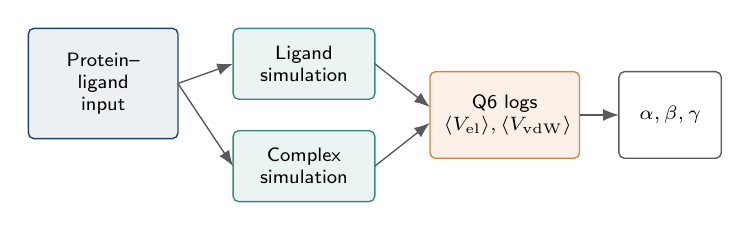
\begin{tikzpicture}[font=\sffamily\fontsize{7.2}{8}\selectfont]
  \definecolor{navy}{RGB}{30,65,110}
  \definecolor{teal}{RGB}{53,137,132}
  \definecolor{orange}{RGB}{214,132,61}
  \definecolor{grayline}{RGB}{90,90,90}

  \draw[rounded corners=2pt, fill=navy!8, draw=navy, line width=0.5pt] (0.0,1.6) rectangle (1.9,3.0);
  \node[align=center,text width=1.5cm] at (0.95,2.3) {Protein--ligand\\input};

  \draw[rounded corners=2pt, fill=teal!10, draw=teal, line width=0.5pt] (2.6,2.1) rectangle (4.4,3.0);
  \node[align=center,text width=1.4cm] at (3.5,2.55) {Ligand\\simulation};

  \draw[rounded corners=2pt, fill=teal!10, draw=teal, line width=0.5pt] (2.6,0.8) rectangle (4.4,1.7);
  \node[align=center,text width=1.4cm] at (3.5,1.25) {Complex\\simulation};

  \draw[-{Latex[length=2mm]}, line width=0.5pt, color=grayline] (1.9,2.3) -- (2.6,2.55);
  \draw[-{Latex[length=2mm]}, line width=0.5pt, color=grayline] (1.9,2.3) -- (2.6,1.25);

  \draw[rounded corners=2pt, fill=orange!12, draw=orange, line width=0.5pt] (5.1,1.35) rectangle (7.0,2.45);
  \node[align=center,text width=1.55cm] at (6.05,1.90) {Q6 logs\\\(\langle V_{\mathrm{el}}\rangle,\langle V_{\mathrm{vdW}}\rangle\)};
  \draw[-{Latex[length=2mm]}, line width=0.5pt, color=grayline] (4.4,2.55) -- (5.1,2.0);
  \draw[-{Latex[length=2mm]}, line width=0.5pt, color=grayline] (4.4,1.25) -- (5.1,1.8);

  \draw[rounded corners=2pt, fill=white, draw=grayline, line width=0.5pt] (7.5,1.35) rectangle (8.8,2.45);
  \node[align=center,text width=1.0cm] at (8.15,1.90) {\(\alpha,\beta,\gamma\)};
  \draw[-{Latex[length=2mm]}, line width=0.5pt, color=grayline] (7.0,1.90) -- (7.5,1.90);
\end{tikzpicture}
\end{tocentry}

\end{document}
